\begin{figure}[H]
\begin{center}
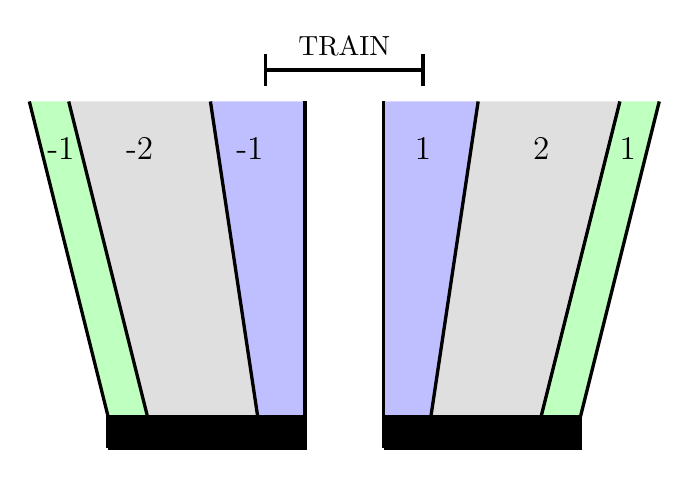
\begin{tikzpicture}

\fill[fill=green!25] (0,0.4) -- (-1,4.4) -- (-0.5,4.4) -- (0.5,0.4) -- (0,0.4); 
\fill[fill=gray!25] (0.5,0.4) -- (-0.5,4.4) -- (1.3,4.4) -- (1.9,0.4) -- (0.5,0.4);
\fill[fill=blue!25] (1.9,0.4) -- (1.3,4.4) -- (2.5,4.4) -- (2.5,0.4) -- (2,0.4);
\fill[fill=black] (0,0) -- (0,0.4) -- (2.5,0.4) -- (2.5,0) -- (0,0);

\fill[fill=green!25] (6,0.4) -- (7,4.4) -- (6.5,4.4) -- (5.5,0.4) -- (6,0.4);
\fill[fill=gray!25] (5.5,0.4) -- (6.5,4.4) -- (4.7,4.4) -- (4.1,0.4) -- (5.5,0.4);
\fill[fill=blue!25] (4.1,0.4) -- (4.7,4.4) -- (3.5,4.4) -- (3.5,0.4) -- (4.1,0.4);
\fill[fill=black] (3.5,0) -- (3.5,0.4) -- (6,0.4) -- (6,0) -- (3.5,0);

\draw[very thick] (0,0) -- (0,0.4) -- (2.5,0.4) -- (2.5,0) -- (0,0);
\draw[very thick] (3.5,0) -- (3.5,0.4) -- (6,0.4) -- (6,0) -- (3.5,0);

\draw[very thick] (2.5,0.4) -- (2.5,4.4);
\draw[very thick] (1.9,0.4) -- (1.3,4.4);
\draw[very thick] (0.5,0.4) -- (-0.5,4.4);
\draw[very thick] (0.0,0.4) -- (-1,4.4);

\draw[very thick] (3.5,0.4) -- (3.5,4.4);
\draw[very thick] (4.1,0.4) -- (4.7,4.4);
\draw[very thick] (5.5,0.4) -- (6.5,4.4);
\draw[very thick] (6,0.4) -- (7,4.4);

\node at (-0.6,3.8) {\large-1};
\node at (0.4,3.8) {\large-2};
\node at (1.8,3.8) {\large-1};



\node at (4,3.8) {\large1};
\node at (5.5,3.8) {\large2};
\node at (6.6,3.8) {\large1};


\draw[very thick] (2,4.8) -- (4,4.8);
\draw[very thick] (2,4.6) -- (2,5);
\draw[very thick] (4,4.6) -- (4,5);
\node at (3,5.1) {\normalsize TRAIN};


\end{tikzpicture}
\caption{Infrared sensor detection zones}
\label{sensorsections2}
\end{center}
\end{figure}